\documentclass[10pt,conference,compsocconf]{IEEEtran}

\usepackage[OT1]{fontenc} 
\usepackage{hyperref}
\usepackage{graphicx}	% For figure environment
\usepackage{subfigure}
\usepackage{titling} % Customizing the title section
\usepackage{dblfloatfix}    % To enable figures at the bottom of page
\usepackage{kantlipsum}     % for random text
\usepackage{todonotes}
\usepackage[margin=0.9in]{geometry}
\usepackage{multirow}
\usepackage[margin=0.9in]{geometry}
\usepackage[english]{babel}
\usepackage{dsfont}
\usepackage[font={small,it}]{caption}
\usepackage{array}
\usepackage{siunitx} 
\usepackage{float}
\restylefloat{table}
\usepackage{mathtools}
\usepackage{pdfpages}

\begin{document}
	
\pretitle{\begin{center}\Huge\bfseries} % Article title formatting
\posttitle{\end{center}} % Article title closing formatting
\title{Bandwidth efficient object recognition for drone swarms}

\author{
	% Your name
	\textsc{Marco Zoveralli} \\
	\normalsize{Semester Project at Laboratory of Intelligent Systems} \\
	% Your supervisors
	%\textsc{Group:}
	%\normalsize{RoadSegmentationFault}\\
	% Your institution
	\normalsize \'{E}cole polytechnique f\'{e}d\'{e}rale de Lausanne
}



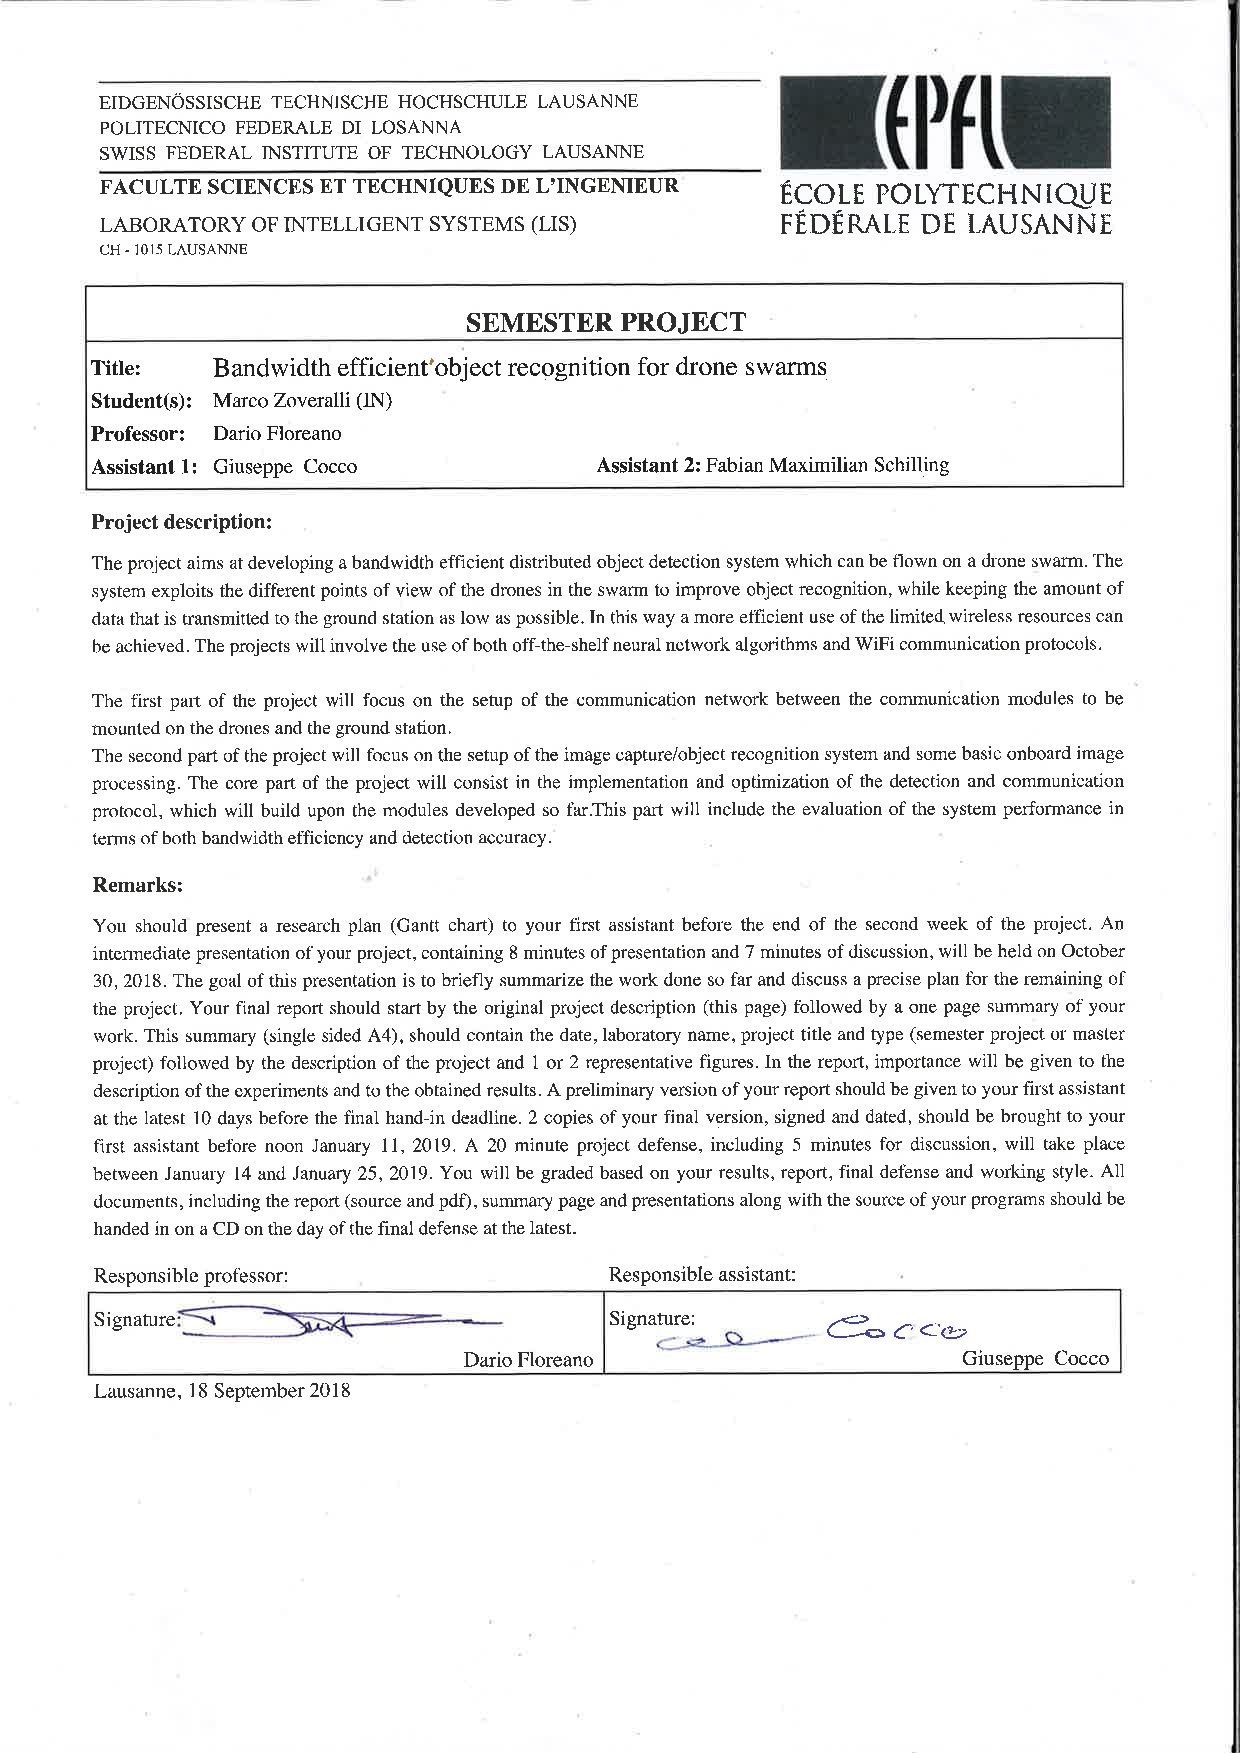
\includepdf[noautoscale]{zoveralliprojectdescription}

\maketitle
TODO: 1-page summary.
\clearpage{}


\begin{abstract}
Getting advantage of multiple devices in order to solve computer vision-related tasks has been a popular choice during the past years. Our main goal is to improve the accuracy of object detection in the context of drone swarms. 
%As additional constraints, we also want to build 
The massive deployment of drones in next generation mobile networks like 5G calls for an efficient bandwidth usage, which is particularly important in the case of multiple co-located drones such as in drone swarms. For this reason we aim at developing a system that minimizes bandwidth usage while enhancing over a single-drone object recognition system.
% in order to converge to a solution and that can behave as an autonomous entity taking decisions and triggering external events.
 We implemented a low-complexity and bandwidth-efficient multi-agent system that takes into consideration the multiple viewpoints and uses them to detect the presence or absence of a target object. We successfully tested the system from the image capture to the intra-swarm communication and data fusion and compared our solution to a single-angent system. Our test results show that the performance of the proposed system in terms of \emph{precision} and \emph{recall} quickly improves with the number of drones while keeping complexity and bandwidth usage low, thus helping scalability.
\end{abstract}

% State of the art: describe the problem and current research.
\section{Introduction}
Object detection can sometimes suffer from non-optimal viewpoints of cameras or low cameras quality. For instance, if an obstruction hides important features of an image that represents a certain object or if an object which is similar to the target one is present in the scene, the prediction could be wrong, i.e.,  false positives and false negatives can occur. The goal of this project is to improve object recognition in the context of drones swarms, in terms of precision and recall measures. In particular, we aim at improving a system that, given a specific object, determines the presence/absence of this object.
%multiple drones in the same swarm, looking at the same point, agree on the presence/absence of the object.
Instead of a single-host system, we exploit the multiple viewpoints available within a swarm. A reliable drone-based distributed object detection system can be either used to trigger an external event (e.g., activating an alarm in case potentially dangerous objects such as suspicious packages or guns are detected in a crowd or also detecting a terrorist suspect in a crowd) or to modify the behavior of the swarm, which is of fundamental importance for it to behave as an autonomous system. We focus on the first setup, which implies having a way to communicate with an external base station that is not part of the swarm, in order to propagate the decision of the group of devices to the external world.\\*
One important constraint that we impose to our solution relates to the usage of bandwidth: it should be kept as low as possible in order to allow scalability and smooth coexistence with systems operating in unlicensed (such as current SMM spectrum) as well as licensed (such as forthcoming 5G networks) systems.
\subsection{Related Work}
Distributed object recognition is a problem that has been studied extensively, from different perspectives.\\*
Rahimpour \textit{et al.} [\ref{reference3}] have proposed a distributed object recognition system in the context of wireless camera networks. Their approach aims at extracting features from each camera, sending them to a base station, and delegate the whole object recognition phase to it. The problem with this solution is that a significant amount of bandwidth is consumed -- even if their histogram compression and feature selection framework are based on Sparse Non-negative Matrix Factorization. Furthermore, their approach is not suited for autonomous drone swarms, in that data fusion is not performed by the nodes capturing the images, but rather by an external one.\\*
In [\ref{reference6}], the authors implemented a swarm-based approach that relies on a cloud system for performing object detection, in a similar fashion as done in [\ref{reference3}]. This requires having a stable internet connection and the possibility of transmitting entire images to another system, which is bandwidth consuming. Also, they did not design a system that emits one final vote based on more the opinion of multiple devices.\\*
Medeiros \textit{et al.} [\ref{reference4}] have proposed an algorithm to aggregate data coming from different cameras and improve object tracking. Their protocol is based on using a distributed Kalman filter  to estimate the position of the object. Unlike the present project, in [\ref{reference4} cooperation is used to improve the tracking of the target object, rather than assessing its presence or absence.\\*
%Saligrama \textit{et al.} [\ref{reference6}] have proposed an algorithm to reach a MAP (maximum a posteriori) estimate consensus in a peer to peer sensor network.\\*
The closest work to our contribution is the paper by Giusti \textit{et al.} [\ref{reference5}]. In [\ref{reference5} the authors have proposed a mechanism to perform distributed recognition of hand gestures through a statistical classifier using a distributed consensus protocol to make the nodes of the network converge to a single decision. The decision process takes into account the quality of the prediction of each node.
%The quality is defined as the certainty that the predicted hand gesture corresponds to the observed one. This approach is the main source of inspiration for our system, for what concerns the communication and consensus protocol.
However, the setup and the goal of their solution differ from ours. In the first place, the goal in the two setups is different, in that the aim in \ref{reference5} is to classify an object that is assumed to be present, while in our case the goal is to reliably decide on the presence of a target object. In the second place, in \ref{reference5} wheeled robots communicate at close distance, and thus do not suffer from severe bandwidth and interference constraints as in the case of wireless communication, which is exacerbated in the case of drones due to the peculiarities of the air-to-ground propagation channel [\ref{reference8}. Finally, in [\ref{reference5}] a Support Vector Machine (SVM) is used for classification, while we adopt a neural network, which better fits the problem we want to address.
% they use infrared, they rely on Support Vector Machine (SVM) classifiers, communication, and they aim at classifying an object that they assumed to be there. Instead, we rely on wifi communication, we use neural network models, and we aim at determining whether a specified object is present or absent.\\*
\section{System Setup}
A general target scenario is the one shown in Figure \ref{fig:setup}.
%\begin{center}
\begin{figure}[h!]
	\centering
	%\captionsetup{type=figure}
	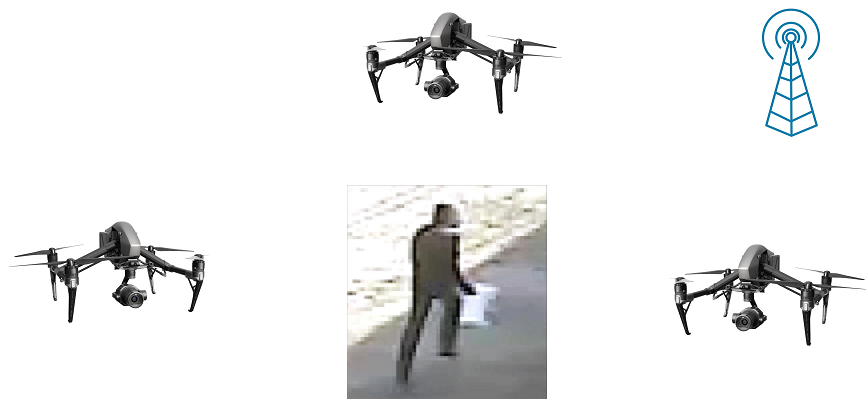
\includegraphics[width=0.47\textwidth]{img/setup.png}
	\caption{System setup}
	\label{fig:setup}
%\end{center}
\end{figure}
Multiple drones, each one with a camera mounted on top of it, point to the same direction and try to understand whether a target object is present. This may be the case, for instance, of a surveillance system in which drones are located along the borders of a square point towards the center of it. Another case of interest is that of a rescue mission in which a drone swarm moves inside a building affected by a fire or leakage of dangerous substances looking for survivors in order to plan a rescue mission. Our approach consists in having these devices communicating in order to share their opinions on the presence or absence of a target object with each other. Each drone runs a local object detection algorithm \footnote{A pre-trained neural network algorithm: \href{https://github.com/tensorflow/models/blob/master/research/object\_detection/g3doc/detection_model_zoo.md}{SSD Mobilenet}, trained on MSCOCO dataset}, but the target object is classified as present if and only if at least a minimum number of predictions is positive about its presence. Our design foresees to have a leader that collects all the predictions of the hosts. The leader takes care of the data fusion ands sends the final result to the base station. More details are provided in section \ref{sec:design}.\\*
Since the swarm of hosts is considered as an independent system, the communication occurs directly between hosts, without any third device as intermediary, which is the case in most WiFi networks. Therefore, the natural choice is to use an adhoc network for exchanging messages between the network nodes. This, together with the fact that the leader changes periodically, allows to avoid single points of failure in the system.
\\*We now give additional information about the setup of our system and the hardware that was involved.
\subsection{Hardware}
\subsubsection{Embedded boards}
The single-board computers that were used in this project were the Odroid XU4. Thanks to the acceptable power of this device \footnote{\url{https://wiki.odroid.com/odroid-xu4/hardware/hardware}}, it is possible to run relatively complex algorithms, including neural networks, in hundreds of milliseconds. Ubuntu MATE is the chosen operating system, which allows to easily run modern software platforms, such as various Python libraries/toolkits and Go. Go is a programming language designed by Google engineers, whose main characteristic is to be simple and powerful \ref{reference9}. The board has three USB interfaces and an ethernet one. Each drone will have one of these devices attached. Any additional piece of hardware, such as connectivity modules or cameras, will be attached directly to this board.
\subsubsection{Connectivity}
The WiFi Module 5 was used in order to provide wifi connectivity among the Odroid boards. The choice of this component is supported by the fact that connectivity tests have shown a positive outcome for the adhoc mode too, which is the WiFi mode that we use to make the nodes of the network communicate.
\subsubsection{Image Acquisition}
Image capture is performed by the OpenMV Cam M7 camera \footnote{\url{https://openmv.io/products/openmv-cam-m7}}. It easily allows the capture of images of various sizes and their transfer to the Odroid. Although some on-camera image processing  can be done with such camera, due to its relatively low computational power this is done on the Odroid, i.e., the OpenMV camera is used only to capture the images. The connection with the board is done via USB.
%\subsection{System Setup}
%The initial, very simple, setup is made of three devices that join an adhoc wireless network. Figure X shows a sketch of this configuration: the nodes communicate directly with each other and their camera points to the same point, where the object is supposed to be. Each node runs a pre-trained neural network algorithm \footnote{\href{https://github.com/tensorflow/models/blob/master/research/object\_detection/g3doc/detection_model_zoo.md}{SSD Mobilenet}, trained on MSCOCO dataset}, thanks to the support of the tensorflow library. Each node in this system performs object detection: in addition to the confidence score, they also provide the bounding boxes of each prediction. Depending on the design of the consensus protocol and of the chosen setup -- which might be different from the described one --, the local prediction may be provided to one or more nodes in the network. This, along with the data aggregation phase, is described in the following section.
%The result of the local prediction of all the nodes is provided to all the other nodes in the network. Then, there is a data aggregation process, during which the nodes agree on the presence or absence of the chosen object.
%During the development phase, the hosts are reached through ethernet connections. The 
\section{Object Detection Setup}
\label{sec:obj_det_setup}
As already mentioned, we use neural networks in order to perform object detection. Although these models perform better than several classifiers, we cannot use too complex algorithms because execution time can become an issue if we consider that each drone must do continuous predictions in order to keep its opinion up-to-date and that our single-board computers do not have the computational power of state-of-the-art computer clusters. Therefore, the idea is to compensate the lack of state-of-the-art networks through the presence of several devices trying to detect the same object.\\*
The same holds for cameras: since we have a swarm we can mount cheaper cameras of lower quality and less weight and still get good performance thanks to the different viewpoints.
\subsection{Image Acquisition}
Two parameters that must be tuned during the image acquisition phase are the capture rate and the frame size.
\subsubsection{Capture rate} it defines how often images are captured and sent to the odroid board. In order to have an accurate prediction, it would be nice to have the interval between two consecutive takes as small as possible (i.e., very high rate), so that the local view is always up-to-date.
However, the prediction rate of the Odroid XU4 imposes a constraint on this, since the capture rate of the camera must be lower than or equal to the prediction rate. Failure in doing this, would result in sending a higher amount of data than that can be handled, which would result in predictions that are not up to date.
\subsubsection{Frame size} it defines how big the taken images are. Ideally, we would like to capture images whose size is similar to the ones that were used to train the neural network, in order to have better performance. However, a larger frame size implies higher computational time as well, which can have a bad impact in terms of the "capture rate vs prediction time" issue. Also, it depends on the camera resolution as well.
In our setup we tested 64x64 and 128x128 images.
\subsection{Model Selection and Preliminary Object Detection Tests}
Among the available pre-trained models, the \href{https://github.com/tensorflow/models/blob/master/research/object\_detection/g3doc/detection_model_zoo.md}{zoo models trained with the COCO dataset} caught our attention, since they offer several alternatives in terms of performance and execution speed. We tested few of them.
At fist glance, it might seem that a classification algorithm would be suitable for our task of detecting the presence of an object.
%It might seem that it does not make sense to perform object detection and that we could use some classifier. 
However, classifiers usually handle -- and are trained with -- simple images with one object. In a real scenario, there would usually be several objects and the target should be detected among them. Traditional classifiers do not handle setups like this.
%This is hardly true, since in any real context the captured images are quite more complex than the ones handled by classifiers: the latters handle simple images with one object, while in a real, complex, scenarios, we would need to detect the presence of an object that we specify among a set of items.
% someone could also argue that SSD mobilenets are at the end not that good. Surely there are better options in terms of accuracy, but they take much more time to give a result. Other alternatives usually consist in classifiers that perform far worse, since they aim at classifying an image (and as we just mentioned, it means dealing with far simples images)
\subsubsection{SSD Mobilenet}
\label{model:ssd}
Performance and computation time vary depending on the image size and on the detected object.
% 2017 model
% 64x64 images: average computation time = 100ms on pc, around 400ms on ODROID
% 128x128 images: average computation time = 120ms on pc, 400ms on ODROID
With 64x64 and 128x128 images, we measured an average computation time on the Odroid boards is around 400 ms. There is no significant difference in terms of computation time, but performance is improved by 128x128 images. Also, since the model was trained with the MSCOCO dataset \footnote{\url{http://cocodataset.org}}, whose samples are 640x480, better performance would be achieved with 128x128 images, since the size is closer to that of the training set.
This should be kept in mind for any future use of our approach: re-training the model might be necessary in order to have better performance.
Since our goal was to develop a system which can handle sub-optimal components, we used the pre-trained neural network and used it out-of-the-box. Such mismatch between the image training set and the size of the images used in the system resulted in very accurate predictions for some kinds of objects \ref{fig:person_detection}, but not so good ones for others \ref{fig:bottle_detection}. Another consequence was that several false negatives are generated for some of these detections. In our experiments we considered classes of objects that proved to be easily detectable under ideal conditions, i.e, they are detected with high confidence score.\\*
Finally, in order to further motivate our setup, figure \ref{fig:person_bad_position} shows that even classes that are detected very well in some conditions (see figure \ref{fig:person_detection}) can be badly recognized if observation conditions change.
%We can notice that with too small images there are several false negatives: although the object is clearly visible, the model is not able to detect the object or it finds it with very low confidence scores (lower than 20\%), as soon as the distance from the object slightly increases. The problem with these image sizes is that even small distances cause the detection algorithm to perform poorly, as the objects cannot be recognized and located.
%One thing that we noticed about this model is that some objects are recognized better than others: for instance, people are detected very well \ref{fig:person_detection}, while objects like bottles are poorly detected \ref{fig:bottle_detection}.
%This should be kept in mind in case of any real use of our ideas: the model should be trained according to what the future application is. Also, it should also be noticed that these models are trained with 640x480 images, while our images are much smaller.
\begin{center}
	\captionsetup{type=figure}
	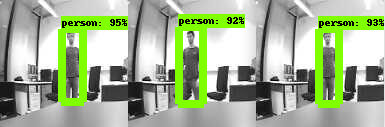
\includegraphics[width=0.47\textwidth]{img/person_detection.png}
	\caption {Preliminary test of detection of people in a noisy environment: the confidence scores are extremely high.}
	\label{fig:person_detection}
\end{center}
\begin{center}
	\captionsetup{type=figure}
	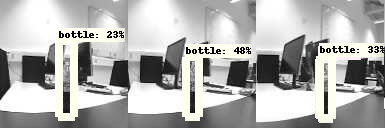
\includegraphics[width=0.47\textwidth]{img/bottle_detection.png}
	\caption {Preliminary test of detection of bottle in a noisy environment: the confidence scores are lower than the ones that relate to people, although the quality of the view is comparable.}
	\label{fig:bottle_detection}
\end{center}
\begin{center}
	\captionsetup{type=figure}
	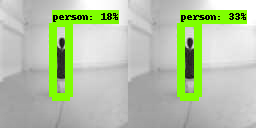
\includegraphics[width=0.30\textwidth]{img/person_bad_position.png}
	\caption {A person not detected very well.}
	\label{fig:person_bad_position}
\end{center}
\subsubsection{Faster R-CNN (Region Convolutional Neural Network}
These models represent the state of the art in terms of accuracy [\ref{reference0}]. However, one big issue relates to the long prediction time, which is around 200 ms on state-of-the-art hardware (NVIDIA Tesla K40 GPU Computing Processor Graphic Cards, as mentioned in [\ref{reference0}]), and therefore it becomes unfeasable to use them on our hardware, which has much lower computational power.
\subsection{Measures of Interest}
Whenever a prediction is performed, the neural network provides a set of output parameters for each object class. Each prediction contains the following information:
\begin{itemize}
\item the class of the object that was localized.
\item the confidence score of the prediction.
\item the area in which the object is located (i.e. the bounding box)
\end{itemize}
Unlike from classification algorithms, here the output is not represented by a vector of probabilities whose sum amounts to 1. In fact, neural networks make several predictions on different regions, which relate to different objects and are therefore independend from each other. Specifically, for each region of the image and for each object class the NN outputs a score indicating the likelihood that the given object is present in the considered region.
%In order to have some insight about the validity of one host's prediction, we would like to have a probability associated to the presence of the object that the system is seeking. We can get this information if we do some reasoning on the bounding boxes that surround the objects. 
One first thought that we had was that, under some assumptions, the size of the bounding boxes might have given some useful information in order to give proper weights to different predictions. The idea was that, if we assume that an object has symmetric features, having a larger bounding box means being closer to an object. While this might be true, some tests we performed on the training dataset showed that the size of the bounding box has a dependency with the confidence which is not easy to be exploited. This is why we are considering the confidence score as the only value involved in the predictions calculation. As the next section \ref{sec:design} shows, we will rely on a mechanism that considers an object as present if a subset of devices (whose size is chosen a priori) considers it as present.
%One assumption that we are making during this project is that the cameras in the network point to the same direction. This implies, for objects with symmetric visual features, that a larger bounding box means that the camera is closer. This gives information in terms of how influent a prediction should be. Figure YYY shows that the highest confidence is reached with a largest bounding box (i.e., smaller distance between camera and object). Alternatively, if an object is not symmetric, the bounding box may still give useful information if the angle of view is the same as the other cameras. This is shown in figure XXX: it is possible to see that the when the examined object has larger bounding box, the confidence score is higher as well. However, this would result in a setup of limited interest. Another problem is that using the bounding box as an estimate of the quality of the prediction can be risky, because the predictions are often noisy and therefore a larger bounding box is not really related to the confidence score value. Therefore, this approach is highly arguable and therefore we focused on the confidence scores given by each hosts, and we aimed at getting advantage from the numerosity of the nodes in the network -- since we are dealing with swarms of devices.
%\subsection{Preliminary Object Detection Tests}
%These are the object labels that we are going to consider during our experiments: person, bottle, monitor, laptop, bycicle, umbrella, skateboard, suitcase.
%Preliminary experiments showed that the chosen model is able to accurately predict the presence of some kinds of objects, such as computer screens. Figure X shows that an optimal point of view allows to get a very high confidence score on this class of objects.
\section{Proposed System}
\label{sec:design}
Designing the protocol was one of the main contributions of this project. Besides being able to improve object detection with respect to a single drone, our goal is also to ensure that little bandwidth is used and that the swarm is able to take a decision as if it was a single, independent, system. The main challenges involved are:
\begin{itemize}
\item how a single object detection prediction is obtained and how it is communicated to other hosts
\item what kinds of messages are transmitted
\item how data is aggregated and combined together
\item how the faults of the network nodes are handled
\item how the information is transferred for external purposes.
\end{itemize}
Our protocol is divided in three different phases, that involve significantly different activities:
\begin{enumerate}
\item capture the image with the camera, and transfer it to the Odroid
\item perform object detection on the Odroid, and propagate the result to the other hosts of the network
\item aggregate information together in order to determine a final prediction
\end{itemize}
\subsection{Consensus Protocol}
Whenever a consensus problem is faced, there are few intuitive approaches that define how the nodes cooperate in order to achieve a result. One way consists in having a leader that takes the local predictions from all the nodes in the network, aggregates the results, takes a final decision, and propagates the final decisions to all the nodes in the network (or to an external entity). An advantage of this approach is that the communication scheme is quite simple: all the nodes provide their prediction to a single node, who is the only one that needs to calculate the final result. This also implies that the bandwidth usage is kept low, since only the leader needs to see other nodes' messages. However, this solution requires that the leader is elected dynamically in case of failures (leader election). Furthermore, there should be some criteria to determine the eligibility of nodes to become leaders (e.g. the node that is able to communicate with more hosts). A second approach would be to have every node to receive all the values and computing the (same) solution. While this ensures robustness (especially against faults), it also means that unnecessary work is performed: the result is the same as the previous approach, with the difference there may be several more messages transmitted between hosts. Finally, a third approach consists in having each node to compute part of the final solution and then all the computations have to be aggregated. This approach is potentially very flexible and smart, because it allows to define very complex data fusion mechanisms.
However, these mechanisms are usually very complex and guarantee better results only under specific conditions.
For instance, many of such systems require a clustering algorithm, which adds complexity and requires communication resources for up-keeping and tracking the rapidly changing network topology and communication conditions of drones swarms.
%Since we are assuming that in our adhoc network every node can communicate directly with all the others, we decided to proceed with the first approach.
We chose the first approach because of its ease of implementation and it is optimal if there is no packet loss. Since in real systems there are packet losses, and for scalability issues, we switch leader at each round, in order to have some spatial diversity in the network.
\subsection{Protocol Overview}
\label{subsec:protooverview}
Our approach got inspired from the family of consensus protocols Paxos. However, our usage is different from the typical ones, which often aim to reach \textbf{state machine replication}. In fact, we want to get advantage of the hosts' predictions just to determine whether the target object is present or not. As a consequence, many of the constraints of classical consensus protocols are relaxed and do not need to be met. The idea is to define a majority (M) as a fraction of the total number of hosts of the network (N). The majority should express a meaningful lower bound in terms of number positive predictions that are needed in order to trigger a positive final prediction. A high majority implies having less false positives, while a low majority will cause less false negatives. We tested M=N/2+1, which is fair in terms of false positives and false negatives, and M=N/3+1, which favors false positives. In theory it would be logical to consider only the former value of M. However, since the models that we are using sometimes fail at detecting true positives with the provided images (as explained in \ref{model:ssd}), it makes sense to have a system that favors positive detections.
\begin{center}
	\captionsetup{type=figure}
	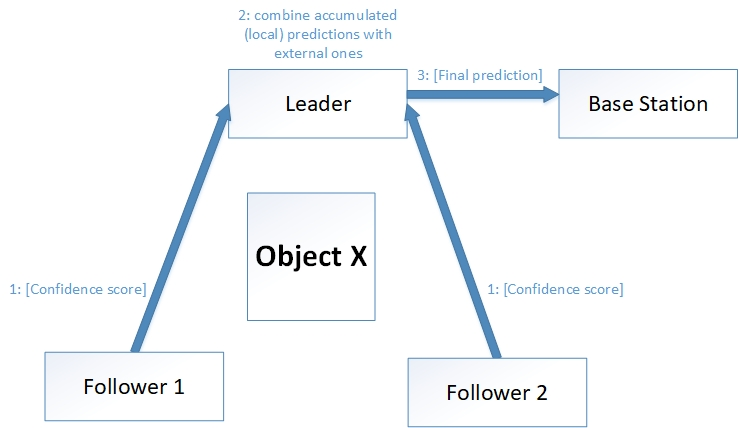
\includegraphics[width=0.47\textwidth]{img/protocol_sketch_inter_host.jpg}
	\caption {Inter-host communication}
	\label{fig:inter_host}
\end{center}
The decision process takes place in rounds: during a round the leader must take a decision that is based on its local prediction and the other hosts' predictions. The leader probes all the other hosts in order to receive their predictions: the transmission of the probe message is repeated periodically (T\textsubscript{probe}) in order to mitigate the impact packet losses. Each host (including the leader) has a timeout (T\textsubscript{timeout}) after which it declares the object as absent (for that round) and it advances to the next round. T\textsubscript{timeout} = K * T\textsubscript{probe}. The leader advances to the next round after a decision for the current round is taken. This implies three cases:
\begin{itemize}
\item Timeout: the object is declared as absent for that round. This occurs if not enough positive predictions are received or if not all predictions are received
\item Predictions from all hosts are received, but there is no positive majority: the object is declared as absent for that round.
\item A majority of positive predictions is received: the object is declared as present for that round.
\end{itemize}
A sketch of the protocol is shown in figure \ref{fig:inter_host}.
\subsection{Prediction Obtainment and Inter-process communication}Once the image is captured by the camera, it is immediately transferred to the Odroid, which allows the usage of Linux and the Tensorflow library. This has a set of benefits, including a broad flexibility in terms of choice of object detection models and language for inter-host communication.\\*
Figure \ref{fig:intra_host} summarizes the computations that occur within a single host.
First, the Odroid takes care of performing object detection. This model runs over a Python process, which uses Tensorflow. Then, we decided to separate the communication phase and to have another process handling it.
Therefore, the prediction is forwarded to a Go process, which takes care of handling any kind of communication with the other hosts. The local communication occurs via a UNIX socket \footnote{\url{http://man7.org/linux/man-pages/man2/socket.2.html}}, which is a simple and reliable way to do inter-process communication. The communication with the rest of the networks occurs via UDP.\\*
The reason behind Go's usage is that this language is much more robust, flexible and scalable than Python, and its concurrency \footnote{Channels: \url{https://www.sohamkamani.com/blog/2017/08/24/golang-channels-explained/}} and networking features make it an excellent choice for building any kind of distributed system.
%The Odroid takes care of performing object detection, through a model \ref{model:ssd} that runs over a Python process. This prediction is then forwarded to a Go process, that takes care of handling any kind of communication with the other hosts. The reason behind this choice is that Go is much more robust, flexible and scalable than Python, and its concurrency and networking features make it an excellent choice for building any kind of distributed system. This is summarized in figure :
\begin{center}
	\captionsetup{type=figure}
	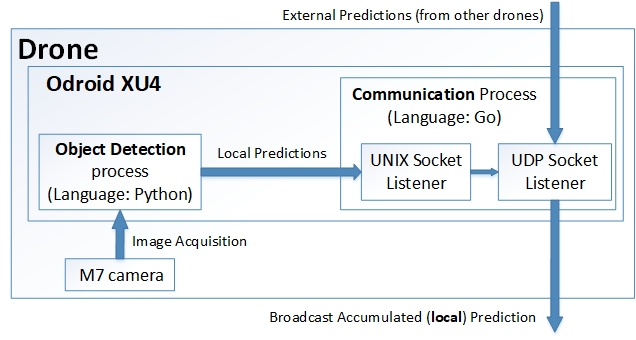
\includegraphics[width=0.47\textwidth]{img/protocol_sketch_intra_host.jpg}
	\caption {Intra-host communication: this figure summarizes the leader perspective, since only the leader takes into account the external predictions, computes a final vote, and propagates it. Follower nodes behave similarly, but they do not compute/send any final vote.}
	\label{fig:intra_host}
\end{center}
\subsection{Exchanged Messages}
There are different kinds of messages that the hosts of our system handle and propagate. They ensure that a final prediction can be obtained and sent to a base station for external usage.
\subsubsection{Probe} it is used to ask for the status of another host. A host propagating a Probe message expects a Status message as reply. Probes have a field indicating the round ID.
\subsubsection{Status} it is used to propagate the status of the host that forwards the message. The status includes the round in which the sending host is, and the current local prediction that relates to the presence/absence of the target object.
\subsubsection{Final Prediction} it contains the final prediction, after considering the other hosts' predictions as well.
\subsubsection{Acknowledgement} a message for confirming the reception of a Final Prediction message.
\subsubsection{Start Round} a message for forcing another host to start a new round. It contains the ID of the round that has to be started.
\subsection{Communication Strategy}We decided to use connectionless communication between hosts (UDP). This allows us to have a lighter communication process, because there is no need to establish and mantain communications between hosts. In order to handle faults and packet losses, each node has some timeout (described above) and resynchronization mechanism (described below).\\*
The final prediction is propagated to a base station, and the leader does not advance to the following round until it is sure that the base station received its message. One sample protocol execution is summarized in figure \ref{fig:temporal_sketch}.
\subsection{Propagation frequency}Since each camera sends frames quite frequently (every 400ms) to the Odroid board -- which runs the object detection algorithm on each of these received frames --, having each network host propagating its decisions as soon as they are performed could cause an explosion of messages in the network. Therefore, each node propagates its decision after being probed. This implies the following advantages: drones' decisions are more reliable, bandwidth usage is reduced, and the resulting protocol is simpler to handle, test and develop.
\subsection{Hosts synchronization}All the nodes that vote in the consensus must be sure that they are voting in the same consensus round as the others. In an ideal environment, with no crashes, faults, and delays, the leader should trigger the beginning of a new round for all the other hosts (with a Start Round message), after it takes a decision for the current round. However, the aforementioned events occur in a real environment. This is why the advancement to a new round can be triggered by other messages as well:
\begin{itemize}
\item Probe message: the receiver updates its status if the received message has higher Round ID that its one.
\item Status message: the receiver updates its status if the received message has higher Round ID that its one. If the received message has lower Round ID, then a probe message with the current Round ID is sent back (here the leader is trying to force the follower to update its round).
\item Start Round message: as described above, it forces a host to start a new round.
\end{itemize}
\subsubsection*{Leader Election}
If we assume that all the nodes have good reachability with each other, it is not important who the leader is. Instead, it is important that the whole swarm does not rely always on the same node to be the leader, in order to avoid a single point of failure. For this reason, the leader is simply determined by the Round ID: each leader has a Node ID, and at round i, the leader is the node with Node ID = i \% N, where N is the number of hosts in our network.
\begin{center}
	\captionsetup{type=figure}
	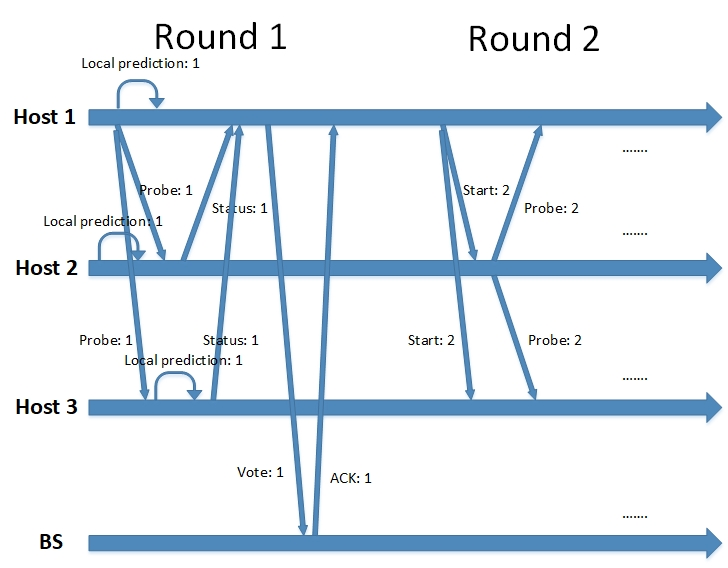
\includegraphics[width=0.5\textwidth]{img/temporal_sketch.jpg}
	\caption {Example of execution of one round of the protocol, without packet losses.}
	\label{fig:temporal_sketch}
\end{center}
\section{Experiments}
In this section we describe the results of our approach, by showing experiments performed on a class of objects.
%We consider two different setups: one that involves a noisy environment and one that was performed in a clean environment without surrounding objects.
We consider a setup that involves a clean environment, without surrounding objects.
Our experiments aim to validate different aspects of our solution:
\begin{itemize}
\item data fusion mechanism
\item communication for the consensus protocol convergence
\end{itemize}
We separated the two procedures, because with the hardware that we had it was hard to fully validate the protocol on a real setup.
\subsection{Data Fusion Validation}
In order to validate the data fusion mechanism we compared our multi-agent system with the single-host system. The measure that we are using relates to the Precision and the Recall. Since Precision = $\frac{TP}{TP+FP}$ and Recall = $\frac{TP}{TP+FN}$, we need two different scenarios (with the same setup, in order to have consistent conditions) to evaluate them.
We assumed to be in an ideal environment. This allowed us to consider an arbitrary number of devices in order to compare the two approaches (single-host system and multi-host system). Let N be the number of hosts that we consider in our system. If N=1, we are in the special case of the single-host system. Let K be the number of different views that we consider for our experiments. For each point of view, we captured some pictures with the camera while it was pointing to the object. The predictions of these pictures are aggregated in the same way as the consensus protocol does for the local prediction process.
In our clean environment, the object could be either what we were looking for, or something else (that could be confused with what we were looking for). In this way, we could compare the two solutions in terms of false positives and false negatives.
This is how the evaluation occurred:
\subsubsection*{Single-host system}There are K samples (one per viewpoint), and the precision and recall are computed on the basis of the outcomes of the predictions on these samples, in the two distinct scenarios.
\subsubsection*{Multi-host system}
Here, the number of samples (from which precision and recall are derived) depends on N.
%We started with a clean setup.
Here, each sample is represented by a set of local predictions from N hosts. This means that for each scenario we have the number of samples that is equal to the combinations of K over N: $\binom{K}{N}$.\\*
Figure \ref{fig:person_FP_FN} shows two views of the setup that we used in order to validate our method: the camera is positioned 3 meters away from the object, and multiple viewpoints are considered. In this particular setup, 9 different viewpoints are considered, on a range of 180 degrees. This means that the angular distance between two viewpoints is 22.5 degrees.
\begin{center}
	\captionsetup{type=figure}
	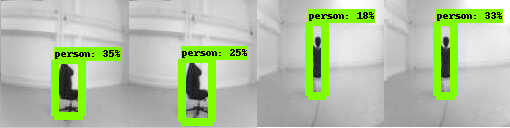
\includegraphics[width=0.5\textwidth]{img/person_FP_FN.png}
	\caption {Setup: we are investigating the presence/absence of a person. In the two leftmost images, a chair is misclassified as a person. In the two rightmost images, a person is not recognized too well.}
	\label{fig:person_FP_FN}
\end{center}
Figure \ref{fig:person_FP_FN_summary_majority2} and \ref{fig:person_FP_FN_summary_majority3} show the comparison between the single-host system (first row of both figures) and our multi-host system in the ideal environment, with M=N/2+1 and M=N/3+1, respectively.
%\begin{center}
\begin{figure*}
	%\captionsetup{type=figure}
	%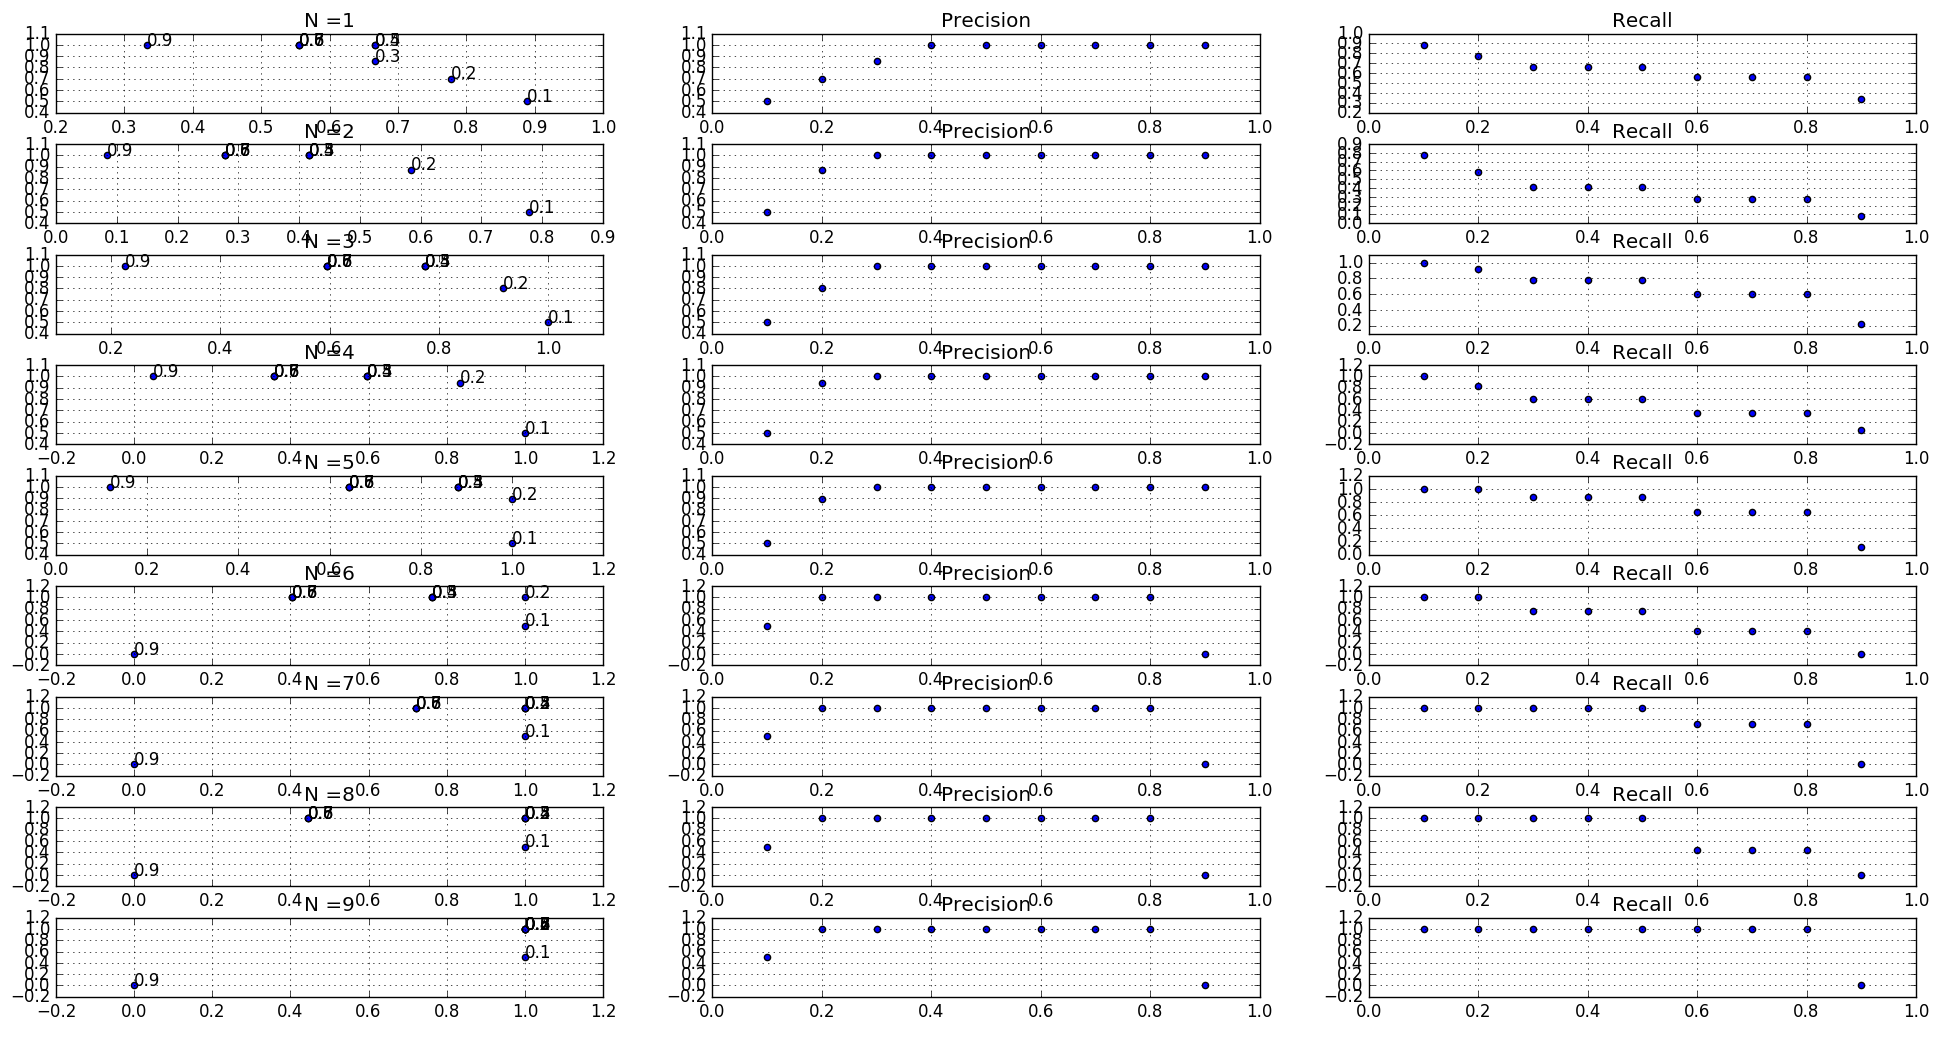
\includegraphics[width=0.5\textwidth]{img/summary_majority_HALF_BIG.png}
	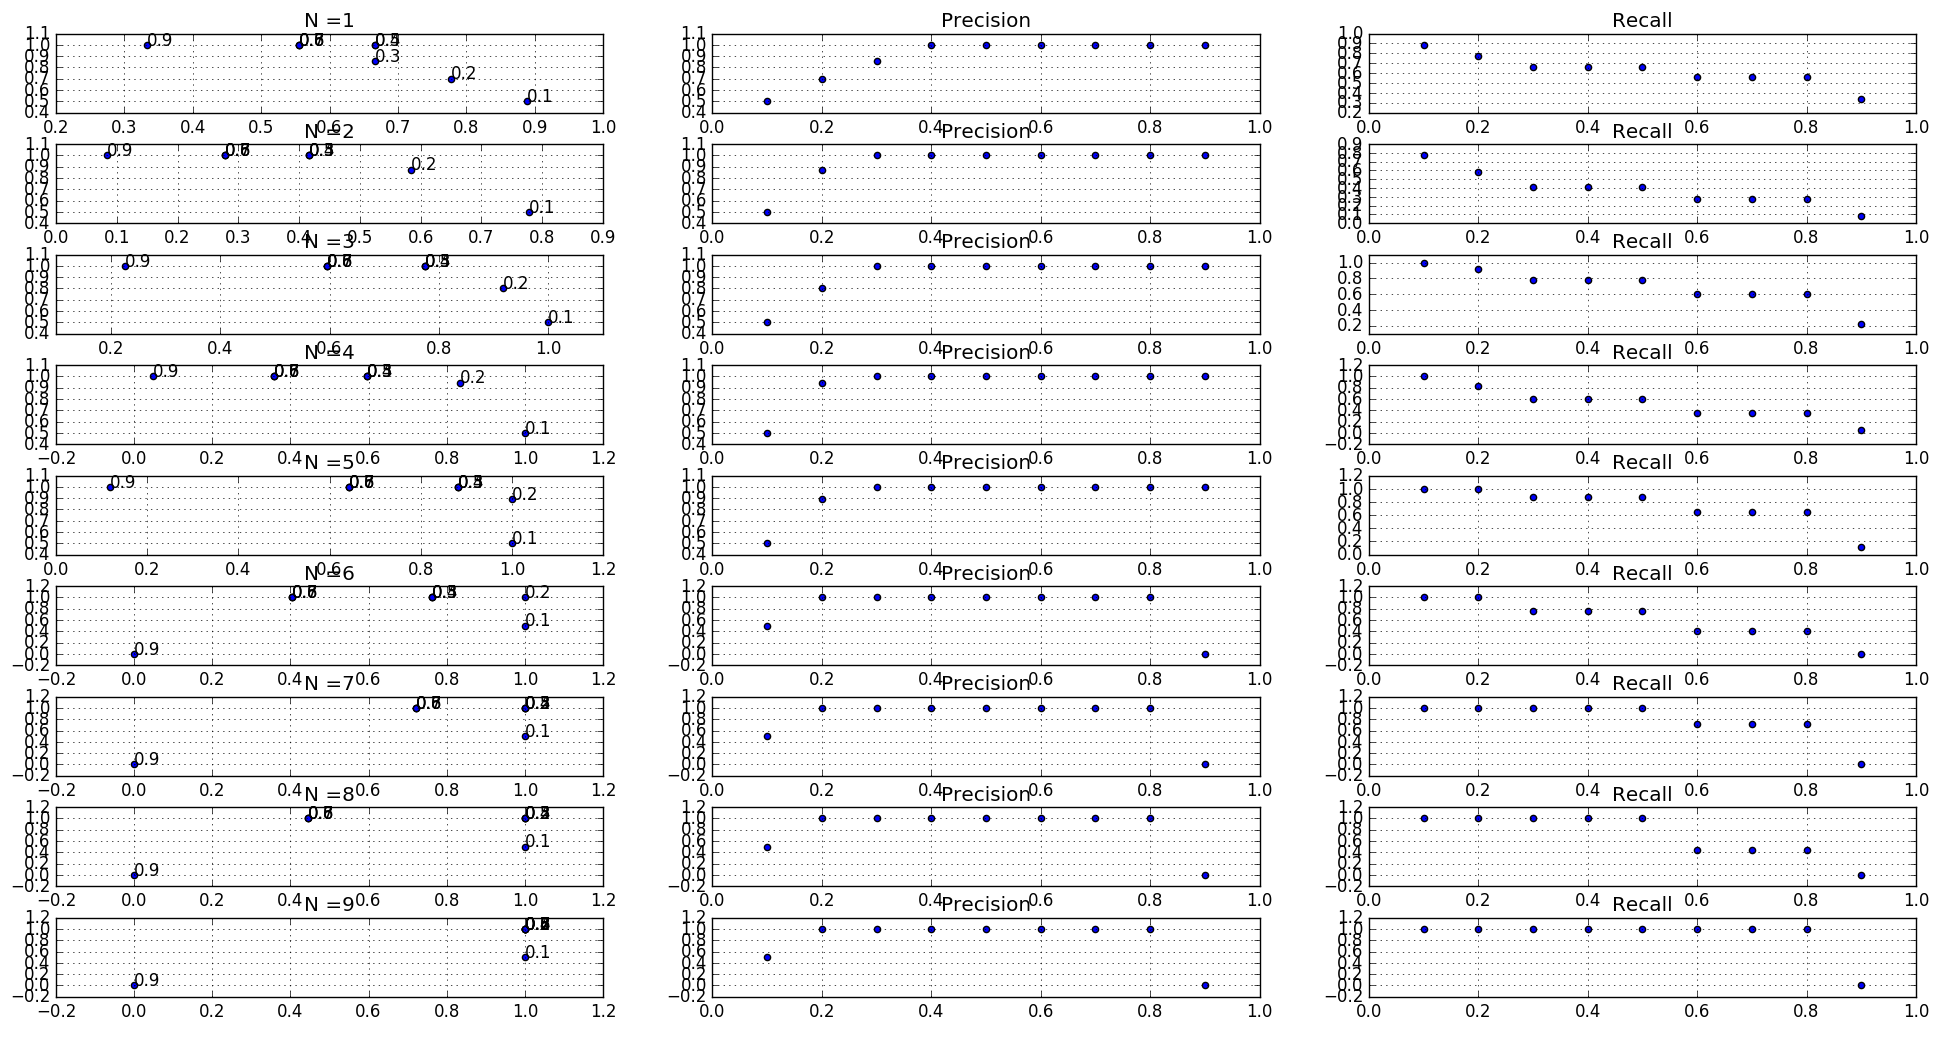
\includegraphics[width=\textwidth]{img/summary_majority_HALF_BIG.png}
	\caption {Majority M = N/2 + 1. This is the number of hosts that need to surpass the threshold with their prediction in order to declare the object as present.}
	\label{fig:person_FP_FN_summary_majority2}
\end{figure*}
%\end{center}
\begin{figure*}
	\captionsetup{type=figure}
	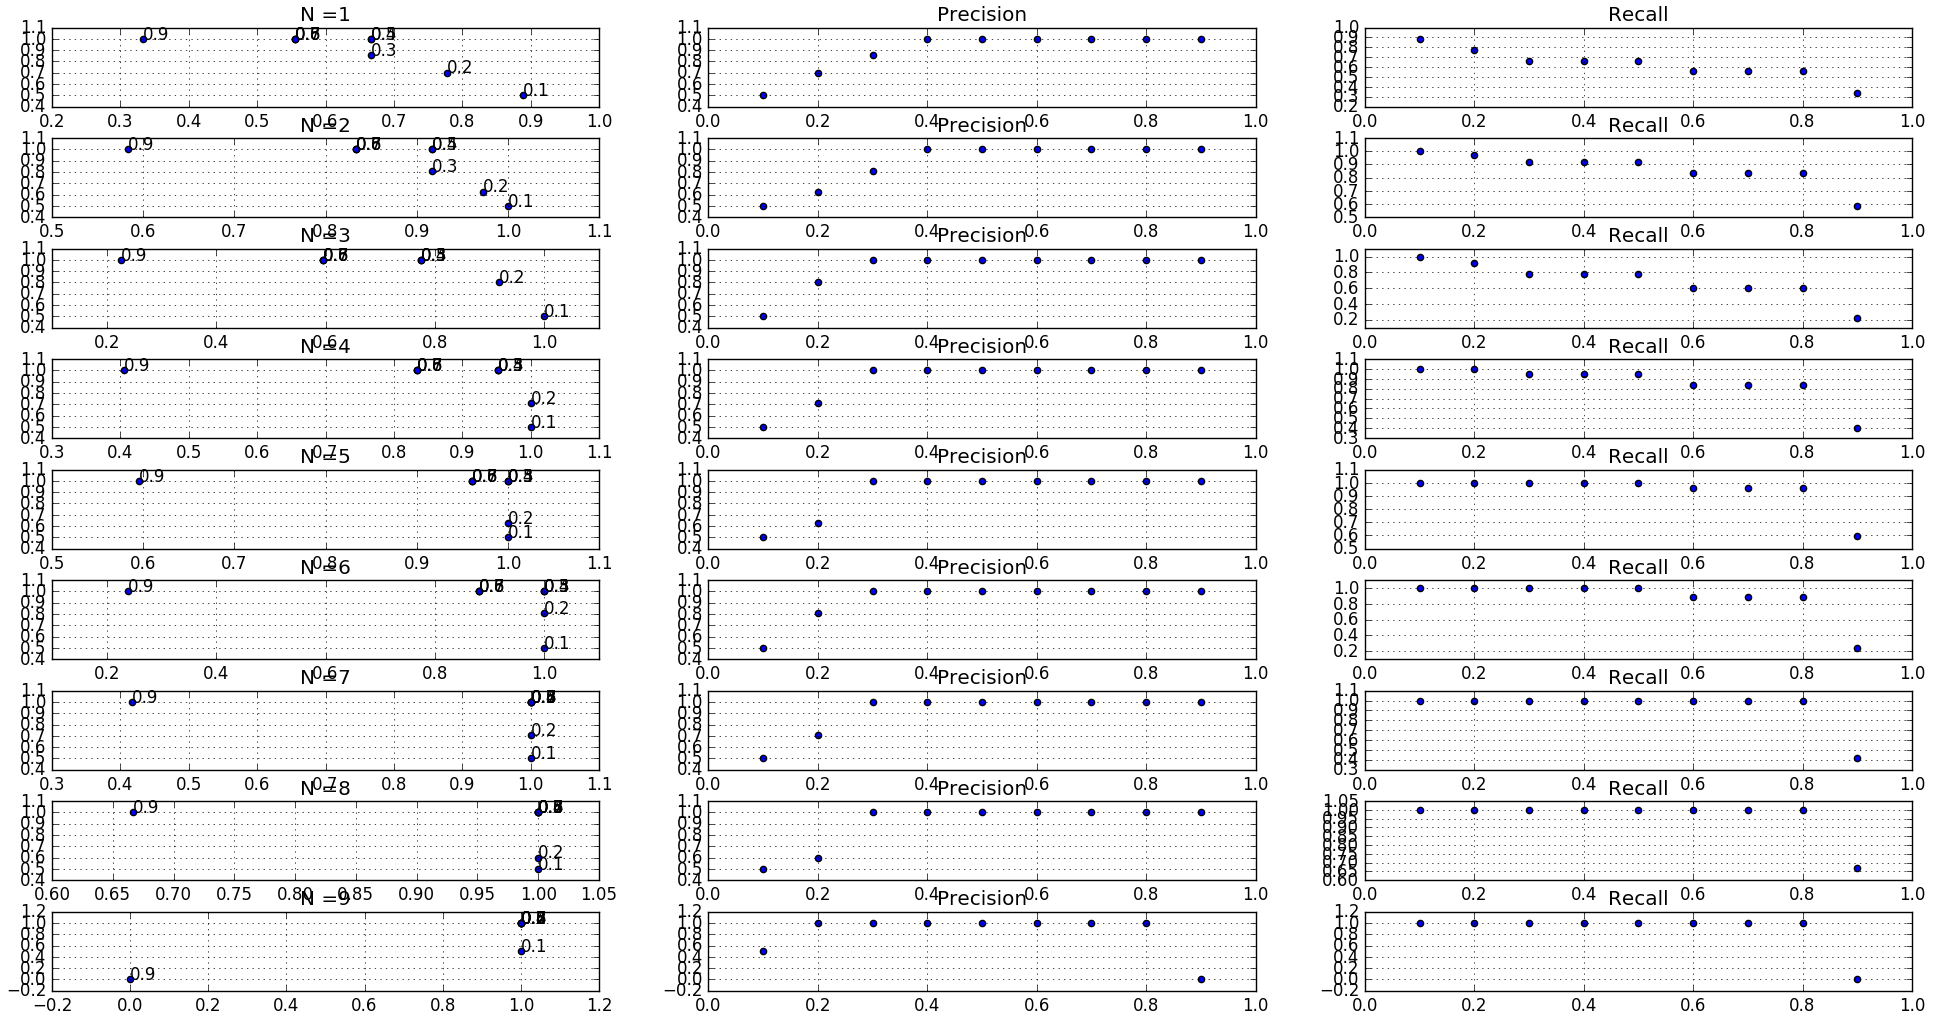
\includegraphics[width=\textwidth]{img/summary_majority_THIRD_BIG.png}
	\caption {Majority M = N/3 + 1. This is the number of hosts that need to surpass the threshold with their prediction in order to declare the object as present.}
	\label{fig:person_FP_FN_summary_majority3}
\end{figure*}
It is interesting to notice that in both cases, under some circumstances, we can find advantages with our approach. The general trend for any system is to have a high precision for high thresholds and a high recall for low thresholds. If a high threshold is picked with the single-host system, we can see that the recalls starts degrading as soon as the threshold goes over 0.2 and 0.3, which are pretty low values. The same reasoning can be done if we decide to pick a low threshold: the recall will benefit from this choice, but the precision is very low for threshold values below 0.3.
If we compare this with the multi-host approach, we can see that the choice of the threshold can be more flexible. In fact, if we pick any threshold, we can see that if the number of hosts in the system is appropriate, we can improve the precision (recall) without degrading the recall (precision) too much.
For instance, if our threshold is 0.4, the single-host system will have a high precision. However, if N=1 we can see that the recall is degraded. If we pick a higher N (e.g. N=6), we can see that the recall has a higher value.
\subsection{Communication and Consensus Test}
In order to test the communication and the convergence of the consensus protocol, we used a setup like the one shown in figure \ref{fig:setup}: there are three drones that point at the center, and they are trying to detect a person. We aim at showing that having a minority of devices (one out three, in this case) that has a non-optimal viewpoint does not impact on the correctness of the system's output.\\*
We firstly put a chair instead of a person, and we saw that two out of three devices detected the absence of a person quite accurately: their confidence score was around 10\%. The third drone's confidence score fluctuated between 30\% and 40\%. During the experiments, we saw that the system was accurately detecting the person as absent although a threshold of 25\% was being used: no false positives.\\*
The same procedure was followed again, but with a person with outstretched arms, and the outcome was similar: two drones were correctly detecting the presence of the person (confidence score between 80\% and 90\%) and one drone with a lower confidence (between 50\% and 60\%). Again, setting the confidence threshold to 80\% did not lead to false negatives.\\*
The test showed that the fully integrated system works properly (image capture and local voting, intra-swarm communication protocol, data fusion and final result transmission).
%\subsection{Methodology}
%Our approach 
%\subsection{Equidistant cameras from different angulations}
%As figure XXX shows, the cameras are pointing in the same direction. Depending on the nature of the object, the detection accuracy is improved in comparison of a single viewpoint prediction. 
%\subsection{Not equidistant cameras from different angulations}
\section{Results}
\label{sec:results}
Here we further discuss the results that we described in the previous section. We can notice that our system, under some conditions, provides better results than a single-host system. In particular, for both the majority values that we tested we had improvements in terms of precision and recall. The best overall performance is obtained with M=N/3+1. The main reason, as already mentioned, is that the models that we are using have more recall issues than precision's, i.e. in general there are more false negatives than false positives.\\*
It can be noticed that there are some cases in which precision and recall fall to 0. This numerical issue is caused by the limited amount of data that we have: we just used 9 different positions for our experimental setup. This implies that if there are not enough optimal views, once the number of hosts that participate in the system is sufficiently high, the majority cannot be reached in any way. This is what happened in our case: among the 9 views that we used for the data fusion validation phase, only 3 of them see a person with more than 90\% as confidence score. This is why for N \textgreater= 6 and M \textgreater= 4 (M=N/2+1), precision and recall will always be 0. Similarly, if M=N/3+1, this will occur for N \textgreater= 8. However, our results also show that, already with a relatively small number of drones, there is at least one threshold value (often a set of values) for which very good performance in terms of precision and recall are obtained.
\section{Conclusion}
\label{sec:conclusion}
We implemented a system that is able to improve object detection accuracy, by getting advantage of multiple views of objects. Our solution is easy to implement, mantain, and extend.
\\*Part of the future work relates to the integration of different models, for object detection, in our system. As mentioned in section \ref{sec:obj_det_setup}, re-training the model for specific applications may improve performance significantly.\\*
Additional improvements could be done on the communication protocol: it would be interesting to extend the system to have independent clusters of devices within the same network. This would imply implementing some kind of distributed routing protocol.
\begin{thebibliography}{1}
\bibitem{IEEEhowto:kopka}
\label{reference0}
S. Ren, K. He, R. Girshick, and J. Sun \emph{Faster R-CNN: Towards Real-Time Object
Detection with Region Proposal Networks}, June 2015.
\vspace*{-0.8\baselineskip}
\bibitem{IEEEhowto:kopka}
\label{reference1}
W. Liu, D. Anguelov, D. Erhan, C. Szegedy, S. Reed, C. Fu, and A. C. Berg \emph{SSD: Single Shot MultiBox Detector}, December 2016.
\vspace*{-0.8\baselineskip}
%\vspace*{-0.8\baselineskip}
\bibitem{IEEEhowto:kopka}
\label{reference2}
A. G. Howard, M. Zhu, B. Chen, D. Kalenichenko, W. Wang, T. Weyand, M. Andreetto, and H. Adam \emph{MobileNets: Efficient Convolutional Neural Networks for Mobile Vision Applications}, April 2017.
\vspace*{-0.8\baselineskip}
\bibitem{IEEEhowto:kopka}
\label{reference3}
A. Rahimpour, A. Taalimi, J. Luo, and H. Qi , \emph{Distributed Object Recognition in Smart Camera Networks}, 2016.
\vspace*{-0.8\baselineskip}
\bibitem{IEEEhowto:kopka}
\label{reference6}
J. Lee, J. Wang, D. Crandall, S. Sabanovic and G. Fox, \emph{Real-Time Object Detection for Unmanned Aerial Vehicles based on Cloud-based Convolutional Neural Networks}, 2017.
\vspace*{-0.8\baselineskip}
\bibitem{IEEEhowto:kopka}
\label{reference4}
H. Medeiros, J. Park, and A. C. Kak, \emph{Distributed Object Tracking Using a Cluster-Based Kalman Filter in Wireless Camera Networks}, 2008.
\vspace*{-0.8\baselineskip}
\bibitem{IEEEhowto:kopka}
\label{reference5}
A. Giusti, J. Nagi, L. Gambardella, and G. A. Di Caro, \emph{Cooperative Sensing and Recognition by a Swarm of Mobile Robots}, 2012.
\vspace*{-0.8\baselineskip}
\bibitem{IEEEhowto:kopka}
\label{reference8}
%A. Giusti, J. Nagi, L. Gambardella, and G. A. Di Caro, \emph{Cooperative Sensing and Recognition by a Swarm of Mobile Robots}, 2012.
B. V. Der Bergh, A. Chiumento and S. Pollin, \emph{LTE in the sky: trading off propagation benefits with interference costs for aerial nodes}, in IEEE Communications Magazine, vol. 54, no. 5, pp. 44-50, May 2016.
\vspace*{-0.8\baselineskip}
\bibitem{IEEEhowto:kopka}
\label{reference7}
T. Mirzayans, N. Parimi, P. Pilarski, C. Backhouse, L. Wyard-Scott, and P. Musilek, \emph{A Swarm-based System for Object Recognition}, 2005.
\vspace*{-0.8\baselineskip}
\bibitem{IEEEhowto:kopka}
\label{reference9}
Kincaid, Jason (November 10, 2009). \emph{Google's Go: A New Programming Language That's Python Meets C++}. TechCrunch. Retrieved January 18, 2010.

%\bibitem{IEEEhowto:kopka}
%\vspace*{-0.8\baselineskip}
%\label{reference6}
%Venkatesh Saligrama, Murat Alanyali, and Onur Savas, \emph{Distributed Detection in Sensor Networks With
%Packet Losses and Finite Capacity Links}, November 2005.
\end{thebibliography}

\end{document}
